\chapter{Progettazione Logica}
A livello concettuale è la fase intermedia tra la progettazione concettuale e la progettazione fisica.
Essa ha diverse fasi:
\begin{itemize}
    \item Richiede di scegliere il modello dei dati - Relazionale
    \item Obiettivo - Definizione di uno schema logico relazionale corrispondente allo
    schema ER di partenza
    \item Aspetti importanti - Semplificazione dello schema per renderlo rappresentabile
    mediante il modello relazionale, ottimizzandolo per aumentare l'efficienza delle
    interrogazioni
\end{itemize}
L'obiettivo primario è quello di tradurre lo schema concettuale in uno schema logico
che rappresenti gli stessi dati in maniera corretta ed efficiente.\\
\paragraph*{Dati in ingresso}
\begin{itemize}
    \item Schema concettuale
    \item Informazioni sul carico applicativo
    \item Modello logico
\end{itemize}
\paragraph*{Dati in uscita}
\begin{itemize}
    \item Schema logico
    \item Documentazione associata
\end{itemize}
Non si tratta di una pura e semplice traduzione, dato che alcuni aspetti non
sono direttamente rappresentabili.
\paragraph*{Esempi} 
\begin{itemize}
    \item Entità $\rightarrow$ Relazione del modello relazionale con gli 
    stessi attributi.
    \item Generalizzazione $\rightarrow$ Dipende dalla situazione!
\end{itemize}
Risulta anche necessario considerare le prestazioni.\\
Qui di seguito lo schema riassuntivo conversione ER $\rightarrow$ Modello relazionale.\\
\begin{table}[h]
    \centering
    \vspace{10pt}
    \caption*{Schema riassuntivo conversione ER - Modello relazionale}
    \begin{tabular}{|c|c|}
        \hline
        \textbf{Modello ER} & \textbf{Modello relazionale}\\
        \hline
        Entità & Relazione (tabella)\\
        \hline
        Relazione & Riferimento (chiave esterna)\\
        \hline  
        Attributo semplice & Attributo (campo)\\
        \hline
        Attributo multivalore & Non presente\\
        \hline
        Generalizzazione & Non presente (conversione in diverse modalità)\\
        \hline
    \end{tabular}
\end{table}
\section{Ristrutturazione dello schema ER}
Eliminazione dallo schema ER di tutti i costrutti che non possono
essere direttamente rappresentati nel modello logico target (relazionale nel
nostro caso).
\begin{itemize}
    \item Eliminazione attributi multivalore
    \item Eliminazione generalizzazioni
\end{itemize}
Inoltre:
\begin{itemize}
    \item Partizionamento/Accorpamento di entità associazioni
    \item Scelta degli identificatori primari
    \item Analisi ridondanze (non dovrebbero esserci)
\end{itemize}
L'obiettivo è quello di semplificare la traduzione e ottimizzare le prestazioni,
teniamo presente che uno schema ER ristrutturato non è più uno schema concettuale nel senso stretto
del termine.\\
Per ottimizzare il risultato abbiamo bisogno di analizzare le prestazioni a questo livello, ma
le prestazioni non sono valutabili con precisione su uno schema concettuale, dipendono dalle
caratteristiche del DBMS, dal volume dei dati e dalla caratteristiche delle operazioni.\\
\subsection*{Indicatori dei parametri di prestazioni}
Consideriamo indicatori dei parametri che regolano le prestazioni:
\begin{itemize}
    \item spazio: numero di occorrenze previste
    \item tempo: numero di occorrenze (di entità e relationship) viste durante un'operazione
\end{itemize}
\subsection{Carico applicativo}
Consideriamo degli indicatori dei parametri che regolano le prestazioni:
\begin{itemize}
    \item Tempo di esecuzione delle operazioni di principale interesse, numero di istanze mediamente
    accedute durante l'esecuzione dell'operazione
    \item Spazio di memoria necessario per memorizzare i dati di interesse
\end{itemize}
Per valutare questi parametri bisogna conoscere oltre allo schema:
\begin{itemize}
    \item Volume dei dati - Numero di istanze previste di entità e relazioni, dimensioni 
    di ciascun attributo
    \item Caratteristiche delle operazioni - Tipo (interattiva o batch), frequenza e dati coinvolti
\end{itemize}
Lo schema di operazione descrive i dati coinvolti in un'operazione, corrisponde al frammento dello
schema ER interessato all'operazione sul quale viene disegnato il cammino logico per accedere alle
informazioni di interesse.
\subsection{Tavola degli accessi}
Con lo schema di operazione si può fare una stima del costo di un'operazione contando
il numero di accessi alle istanze di entità e relazioni, il risultato può
essere riassunto in una tavola degli accessi.
\begin{table}[h]
    \centering
    \begin{tabular}{|c|c|c|c|}
      \hline
      Concetto & Costrutto & Accessi & Tipo \\
      \hline
      & & & \\
      \hline
    \end{tabular}
    \caption{Tavolta degli accessi}
    \label{tab:four-columns}
  \end{table}
  Il tipo distingue gli accessi in scrittura (S) e in lettura (L), le operazioni
  di scrittura sono in genere più onerose (esecuzione in modo esclusivo, aggiornamento degli
  indici).\\
  Solitamente per produrre la tavola di accessi si fa riferimento allo schema di navigazione, cioè
  la parte dello schema ER interessata dall'operazione estesa con delle frecce che indicano in che modo 
  l'oerazione naviga i dati.
\subsection{Tavola dei volumi}
Specifica il numero stimato di istanze per ogni entità E e associazione R dello schema, i valori sono 
necessariamente approssimati, ma indicativi. Il numero medio di partecipazioni di una istanza di entità
alle istanze di relazione dipende dalla cardinalità delle relazioni.\\
I volumi sono quindi influenzati da:
\begin{itemize}
    \item Cardinalità dello schema
    \item Numero medio di volte che le istanze delle entità partecipano alle relazioni
\end{itemize}
Il numero delle istanze si ricava dalla tavola dei volumi mediante semplici operazioni.
\subsection{Analisi delle ridondanze}
Una ridondanza in uno schema ER è una informazione significativa ma derivabile da altre, in
questa fase si decide se eliminarle o tenerle.\\
Ci sono sia vantaggi che svantaggi nel mantenere delle ridoondanze:
\begin{itemize}
    \item Vantaggi - Semplificazione delle interrogazioni
    \item Svantaggi - Maggiore occupazione di spazio, aggiornamenti più pesanti
\end{itemize}
\paragraph*{Forme di ridondanza}
\begin{itemize}
    \item Attributi derivabili da altri attributi della stessa entità o di altre entità o relazioni
    \item Associazioni derivabili dalla composizione di altre relazioni in presenza di cicli
\end{itemize}
\'E necessario considerare la semantica della relazione coinvolta nel ciclo, perchè in casi simili potrebbero
esserci delle ridondanze che non sono tali.
\paragraph*{Esempio slide 35 Docenza - Tesi}
\section{Eliminazione gerachie}
Il modello relazionale non supporta la rappresentazione diretta delle generalizzazioni,
mentre entità e relazioni sì, quindi si eliminano le gerarchie sostituendole con 
entità o relazioni.\\
Ci sono tre possibilità:
\begin{enumerate}
    \item Accorpamento delle figlie della generalizzazione nel genitore
    \item Accorpamento del genitore della generalizzazione nelle figlie
    \item Sostituzione della generalizzazione con relazioni
\end{enumerate}
\subsection{Accorpamento delle figlie nel genitore}
\begin{itemize}
    \item Le entità figlie sono eliminate e al loro posto viene creato un attributo che le rappresenta
    nell'entità padre (un attributo per distinguere il tipo, quale figlia è o nessuna)
    \item Gli attributi della figlia vengono spostati nel padre
    \item Gli attributi che  provengono dalla figlia possono essere nulli
    \item Le relazioni che provengono da una sola figlia hanno cardinalità minima pari a 0
\end{itemize}
\paragraph*{Pro e Contro}
\begin{itemize}
    \item Vantaggi - Accesso contestuale agli attributi del padre e della figlia
    \item Svantaggi - Si ha spreco di memoria per i valori nulli
\end{itemize}
\paragraph*{Attenzione} Se ci sono attributi specifici nelle figlie non si posson
accorpare nel padre, in questo caso è meglio produrre delle relazioni aggiuntive.
\subsection{Accorpamento del genitore nelle figlie}
\begin{itemize}
    \item L'entità padre si elimina 
    \item Gli attributi, le associazioni e l'identificatore del padre sono aggiunti alle figlie
    \item Ogni associazione definita sul padre genera una associazione distinta per ogni figlia
\end{itemize}
\paragraph*{Pro}
\begin{itemize}
    \item Migliore se si effettuano prevalentemente operazioni solo su istanze di una classe figlia
    \item Non ci sono di principio valori nulli
\end{itemize}
\paragraph*{Contro}
Possibile solo se la generalizzazione è totale, dato che non si possono rappresentare istanze
che non sono in nessuna delle classi figlie.
\subsection{Sostituzione della generalizzazione con relazioni}
\begin{itemize}
    \item Si introduce una relazione uno-a-uno fra l'entità padre e ciascuna entità figlia
    \item Occorre inserire il vincolo che ogni istanza dell'entità padre può partecipare solo ad 
    una relazione di legame con le entità figlie
    \item Se la generalizzazione è totale ogni istanza dell'entità padre partecipa necessariamente ad una
    (sola) delle relazioni di legame con le figlie
\end{itemize}
\paragraph*{Pro}
\begin{itemize}
    \item Conviene quando la generalizzazione non è totale e ci sono operazioni
    che fanno distinzione fra le entità padre e figlie
    \item Non è necessario introdurre valori nulli
    \item Genera entità con pochi attributi (le tabelle corrispondenti sono più piccole
    e più tuple possono essere gestite in memoria principale)
\end{itemize}
\paragraph*{Contro}
\begin{itemize}
    \item Si incrementa il numero di accessi per mantenere la consistenza delle istanze rispetto
    ai vincoli introdotti
\end{itemize}
La scelta fra le alternative si può fare con metodo simile a quello visto per l'analisi
delle ridondanze (però non basato solo sul numero degli accessi).
\paragraph*{Regole generali}
\begin{itemize}
    \item \textbf{Accorpamento delle figlie della generalizzazione nel genitore} conviene se gli accessi
    al padre e alle figlie sono contestuali
    \item \textbf{Accorpamento del genitore nelle figlie} conviene se gli accessi alle figlie sono distinti e
    solo se la generalizzazione è totale
    \item \textbf{Sostituzione della generalizzazione con relazioni conviene} se gli accessi alle entità figlie
    sono separati dagli accessi al padre
\end{itemize}
Sono possibili anche soluzioni ibride, soprattutto in gerarchie a più livelli.
\subsection{Note pratiche}
L'accorpamento nel padre è sempre applicabile, ma è sconsigliato in presenza di
elevato numero di relazioni e/o attributi provenienti dalle entità figlie (necessità
vincoli di integrità).\\
L'accorpamento nelle figlie è applicabile solo se la generalizzazione è totale, è
sconsigliabile applicare questa tecnica per una copertura parziale.\\
La tecnica non è adatta per coperture sovrapposte dato che risulterebbe difficile
gestire degli identificatori duplicati relative alle istanze comuni a più entità figlie.\\
Mentre per quanto riguarda la creazione di relazioni, è la soluzione più semplice, sempre applicabile, 
ma può essere dispendiosa per ricostruire l'informazione di partenza.
\section{Partizionamento/accorpamento di entità e relationship}
Ristrutturazioni effettuate per rendere più efficienti le operazioni in base a un
semplice principio:
\paragraph*{Gli accessi si riducono}
\begin{itemize}
    \item Separando attributi di un concetto che vengono acceduti separatamente
    \item Raggruppando attributi di concetti diversi acceduti insieme
\end{itemize}
\paragraph*{Casi principali}
\begin{itemize}
    \item Partizionamento verticale di entità
    \item Partizionamento orizzontale di relationship
    \item Accorpamento di entità/relationship
\end{itemize}
\subsection{Accorpamento di entità}
Due entità legate da una associazione possono essere fuse in un'unica entità
contenente gli attributi di entrambe quando le operazioni fanno sempre riferimento a tutti gli 
attributi delle due entità. In questo modo si risparmiano gli accessi per recuperare i dati
attraverso la relazione che lega le due entità.\\
Si effettuando per associazioni uno a uno.
\section{Eliminazione di attributi multivalore}
Il modello relazionale non consente la rappresentazione di attributi multivalore, si crea quindi
una relazione che collega l'entità dell'attributi designato con una nuova relazione rappresentante 
l'attributo multivalore. La cardinalità sarà uno a molti (dato che ogni entità avrà una sola
istanza dell'attributo multivalore trasformato in entità associato).
\section{Scelta degli identificatori principali}
Operazione indispensabile per la traduzione nel modello relazionale.
\paragraph*{Criteri}
\begin{itemize}
    \item Assenza di opzionalità (NO valori nulli)
    \item Semplicità (preferebza agli identificatori interni, dimensioni ridotte)
    \item Utilizzo nelle operazioni più frequenti o importanti
    \item Se nessuno degli identificatori soddisfa i requisiti precedenti si introducono
    nuovi attributi (codici) contenenti valori speciali generati appositamente per questo scopo
\end{itemize}
\section{Traduzione verso il modello relazionale}
Idea di base: le entità diventano relazioni sugli stessi attributi e le associazioni
(ovvero le relazioni ER) diventano relazioni sugli identificatori delle entità coinvolte
(più gli attributi propri).
\subsection{Entità}
Una entità diviene una relazione definita sugli stessi attributi e con chiave uguale
all'identificatore.
\subsection{Associazioni}
Ogni associazione è tradotta con una relazione con gli stessi attributi, cui si
aggiungono gli identificatori di tutte le entità che essa collega (FOREIGN KEY).\\
Gli identificatori delle entità collegate costituiscono una superchiave. La chiave
dipende dalle cardinalità massime delle entità nell'associazione. Le cardinalità minime
determinano, a seconda del tipo di traduzione effettuata, la presenza o meno di valori nulli e quindi
incidono su vincoli e occupazione inutile di memoria.
\subsection{Nomi delle chiavi}
Non è necessario mantenere per gli attributi chiave della relazione che traduce l'associazione gli
stessi nomi delle chaivi delle relazioni referenziate, si possono scegliere nomi più espressivi
per gli attributi chiave della relazione che rappresenta la relationship.
\paragraph*{Esempio} Se nell'entità progetto ho una chiave denominata "Codice" la
relazione PartecipazioneProgetto avrà una chiave denominata "CodiceProgetto" e non "Codice",
così da risultare ancora più chiaro il riferimento.
\subsection{Relazioni molti a molti}
In questo caso è necessario trasformare la relazione in una relazione con una chiave
nel modello relazionale e inserire i relativi vincoli di integrità referenziale fra le
entità a cui era collegata la relazione nello schema ER.\\ 
Nel caso di relazioni con più entità collegate si crea una chiave esterna per ogni entità
collegata.
\subsection{Relazioni uno a molti}
In questo si accorpa la relazione con l'entità che ha cardinalità massima uno e si crea
una chiave esterna per collegare l'entità con cardinalità massima uno con l'entità
con cardinalità massima molti. Nel caso di cardinalità 0,1 si avrà l'attributo chiave esterna che può essere NULL.
\subsection{Entità con identificatore esterno}
Un identificatore esterno rappresenta un vincolo di integrità referenziale, quindi è 
necessario rappresentarlo nel MR tramite la creazione di chiave esterna che però costituiranno
insieme a un o più attributi chiave primaria della relazione.
\paragraph*{Esempio a cascata}
\begin{figure}[h]
    \centering
    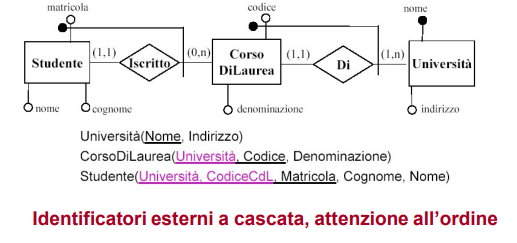
\includegraphics[width=0.5\textwidth]{identificatori_esterni_a_cascata}
    \caption{identificatori esterni a cascata}
    \label{fig:id-esterni-cascata}
\end{figure}
\subsection{Relazioni uno a uno}
In questo caso si accorpa la relazione in un'entità, si sceglie di solito quella con con cardinalità 1-1 dato
che nel caso 0-1 la partecipazione alla relazione è opzionale e quindi si avrebbe un valore NULL.\\
Nel caso di relazioni dove entrambe le entità hanno cardinalità 0-1 si può introdurre una relazione aggiuntiva, 
in modo tale da rappresentare la partecipazione opzionale in entrambi i casi, senza avere valori nulli
sugli attributi (però si introduce una relazione in più). Oppure indicare che le chiavi esterne e gli attributi
della relazioni possono essere nulli.
\section{Documentazione degli schemi logici}
Si devono documentare i vincoli di integrità referenziale, in modo tale da produrre un diagramma con
collegamenti fra relazioni (utili anche per visualizzare i cammini di join).

